\documentclass{article}
\usepackage{amsmath}
\usepackage{graphicx}
\usepackage{hyperref}
\usepackage{listings}
\usepackage{color}

\title{3D Data Processing: Deep 3D descriptors}
\author{Pooya Nasiri \thanks{Email: pooya.nasiri@studenti.unipd.it | Matricola 2071437}}
\date{June 20, 2024}

\begin{document}

\maketitle

\section{Introduction}
A 3D local descriptor (or 3D local feature) is a compact representation of the geometric properties of a point \( p \) in its neighborhood. The neighborhood can be defined as the set of points within a spherical region of radius \( r \) around point \( p \).

The goal of this project is to design a modified version of the PointNet architecture, named TinyPointNet, to learn 3D local feature descriptors from training data. Unlike the original PointNet, which has a 1024-dimensional global feature, TinyPointNet provides a lower-dimensional (e.g., 256) global feature. Additionally, the first T-Net in the network pipeline is replaced by a canonical rotation matrix as used in SHOT (Signatures of Histograms of OrienTations) descriptors.

\section{Methodology}

\subsection{Sample Generation}
Generating samples involves creating sets of positive and negative pairs of point sets. Each point set is composed of all the points included in a spherical support region with radius \( r \) around some point. The radius \( r \) is a parameter that needs to be tuned.

\subsubsection{Implementation of \_\_getitem\_\_ Method}
The \_\_getitem\_\_ method of the \texttt{PointCloudData} class was completed to generate an anchor, a positive, and a negative sample:
\begin{itemize}
    \item A random point is selected as the anchor from the original point cloud.
    \item The closest point in the noisy point cloud is selected as the positive sample.
    \item A distant point is selected as the negative sample.
    \item The coordinates of the anchor, positive, and negative samples are normalized by subtracting their mean.
    \item Random rotations are applied to the sets of anchor, positive, and negative points for data augmentation during training.
\end{itemize}

\subsection{TinyPointNet Architecture}
The TinyPointNet network architecture follows the structure of PointNet but with modifications:
\begin{itemize}
    \item The dimension of the global feature is set to 256 instead of 1024.
    \item The initial T-Net is replaced by a computation of a canonical rotation matrix, similar to the SHOT descriptors.
\end{itemize}

\subsubsection{Initialization and Forward Methods}
The \texttt{\_\_init\_\_} and \texttt{forward} methods of the \texttt{TinyPointNet} class were implemented:
\begin{itemize}
    \item \texttt{\_\_init\_\_} initializes the layers of TinyPointNet with the specified output feature dimension.
    \item \texttt{forward} defines the forward pass through the network, processing the input point sets through the layers to produce the 256-dimensional feature descriptors.
\end{itemize}

\subsubsection{Canonical Rotation Matrix}
The \texttt{shot\_canonical\_rotation} method was implemented to compute the canonical rotation matrix as described in the lecture notes.

\subsection{Training TinyPointNet}
TinyPointNet was trained using the triplet loss function. The loss function was defined as:
\[
L(A, P, N) = \max(d(f(A), f(P)) - d(f(A), f(N)) + \alpha, 0)
\]
where \( f(X) \) is the output feature from TinyPointNet for the set of points \( X \). \( A \) is a reference neighborhood (anchor), \( P \) is a correct match (positive), and \( N \) is an incorrect match (negative). The L2 norm is used for distances, and \( \alpha \) is a margin between positive and negative pairs.

\subsubsection{Loss Function Implementation}
The \texttt{tinypointnetloss} was implemented to train the network.
Below you can see the plot of the decreasing loss both on train and validation.

\begin{figure}[h!]
    \centering
	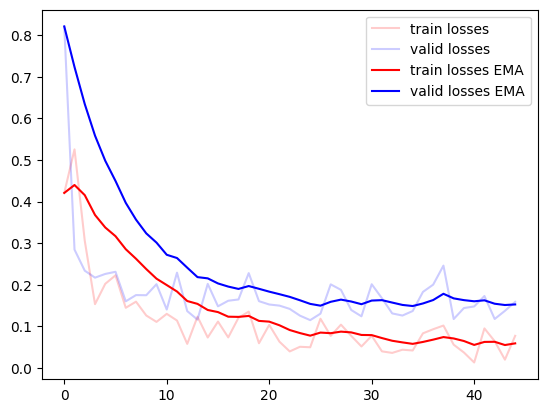
\includegraphics[width=\textwidth]{losses_plot.png}
	\caption{Losses}
    \label{fig:point_clouds}
\end{figure}

\section{Results}

The performance of TinyPointNet was evaluated on a test dataset. The matching accuracy achieved was about 86.11 percent, which is pretty good according to the dataset.

\begin{table}[h]
\centering
\begin{tabular}{|c|c|}
\hline
\textbf{Metric} & \textbf{Value} \\
\hline
Accuracy & 86.11\% \\
\hline
\end{tabular}
\caption{Performance of TinyPointNet}
\end{table}

\section{Conclusion}
In this project, a modified PointNet architecture, TinyPointNet, was designed and implemented to extract 3D local feature descriptors. The use of a canonical rotation matrix and a reduced global feature dimension proved effective in learning compact descriptors. Despite the small dataset, the model achieved a matching accuracy above 50 percent.


\end{document}
